\subsection{Proposed method}
\label{section:proposed_method}
The proposed method combines information from the 2D RGB images and  the depth images. It finds the 3D transformation matrix from one view to another directly in the 3D space by matching known keypoints. This method is built in several steps:

\begin{enumerate}
    \item \nameref{section:charuco_board_corners}
    \item \nameref{section:creation_3d_pc_corners}
    \item \nameref{section:3d_rigid_transformation}
\end{enumerate}

\begin{figure}[H]
    \centering
    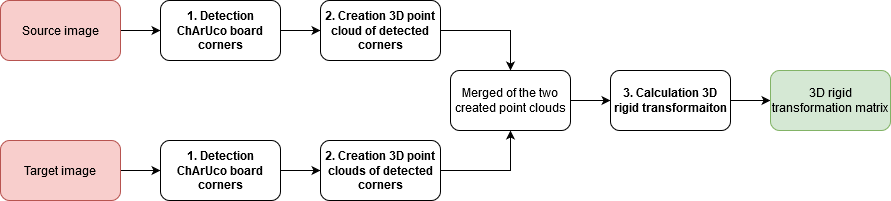
\includegraphics[width=0.95\textwidth]{images/registration/registration.png}
    \caption{Pipeline of the proposed method to find the rigid tranformation matrix}
    \label{figure:registration}
\end{figure}

\subsubsection{Detection of a ChArUco board corners}
\label{section:charuco_board_corners}
To obtain a precise registration, accurate and easy to detect keypoints have to be recognised in the field of view of the different cameras. ArUco markers and chessboards are very useful due to their fast detection and their versatility. The algorithm to detect the corners of the chessboard was developed by \cite{harris_combined_1988}.

The detection and generation of ArUco markers were developed by \cite{garrido-jurado_automatic_2014}. ArUco markers have the advantage of having a unique identification number by pattern. It makes ArUco board versatile and permissive to occlusion. Therefore matching these markers viewed by different cameras is straightforward. On the other hand, the accuracy of their corner positions is not high enough \footnote{According to the OpenCv documentation: \url{https://docs.opencv.org/4.2.0/df/d4a/tutorial_charuco_detection.html}}.

By comparing with ArUco markers, the corners of chessboard patterns can be refined more accurately. Each corner is surrounded by two squares which increases the accuracy of the corner position. However, such a board is less versatile and is not permissive to occlusion.

The benefits of these two different boards are combined in a ChArUco board, figure \ref{figure:charucodefinition}. OpenCV library is used to handle the detection of the corners.

\begin{figure}[H]
    \centering
    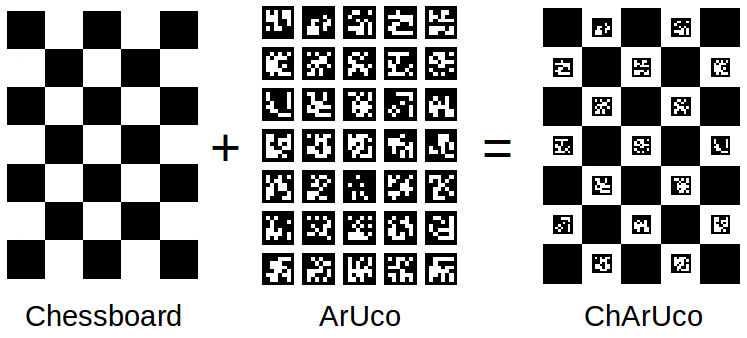
\includegraphics[width=0.65\textwidth]{images/registration/charucodefinition.png}
    \caption{ChArUco board definition}
    \label{figure:charucodefinition}
\end{figure}

A tripod with a ChArUco board is placed in the centre of the scene. It has to be in the field of view of both cameras. The positions in pixel of the detected chessboard corners are recorded for both views. The average over about 50 frames is calculated to be robust to outliers and is saved for the second step.

\begin{figure}[H]
\centering
  \begin{subfigure}[b]{0.48 \textwidth}
    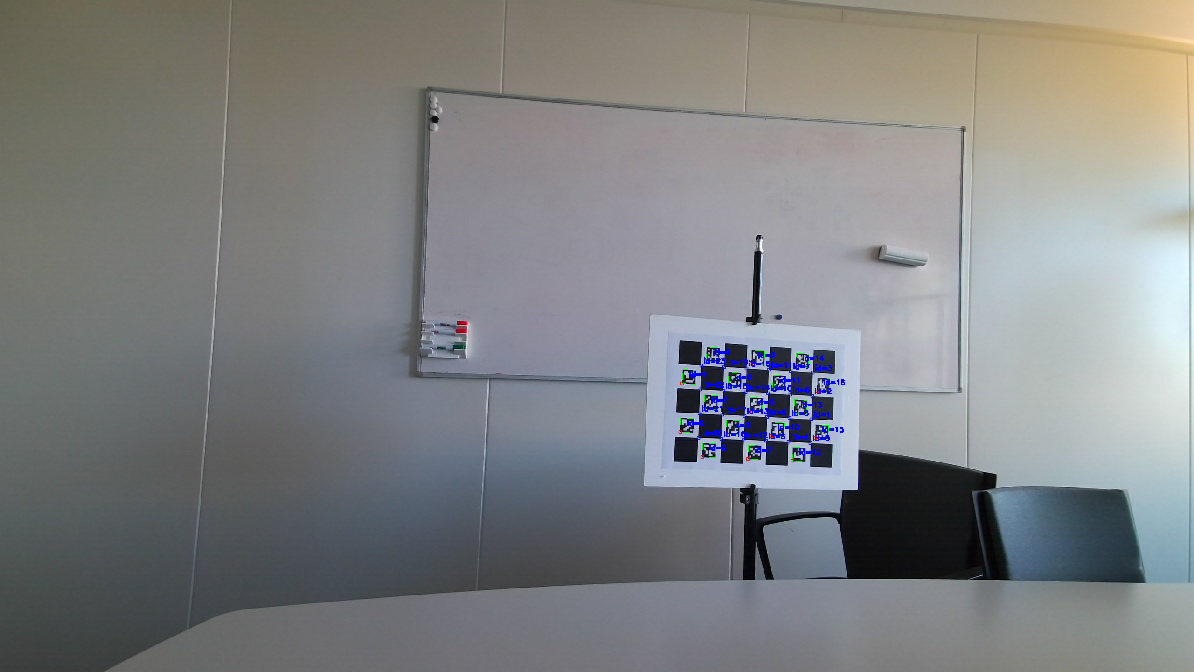
\includegraphics[width=\textwidth]{images/registration/imgr_board_detected.png}
    \caption{Chessboard detection on the right}
    \label{figure:imgr_board_detected}
  \end{subfigure}
  \hfill
  \begin{subfigure}[b]{0.48 \textwidth}
    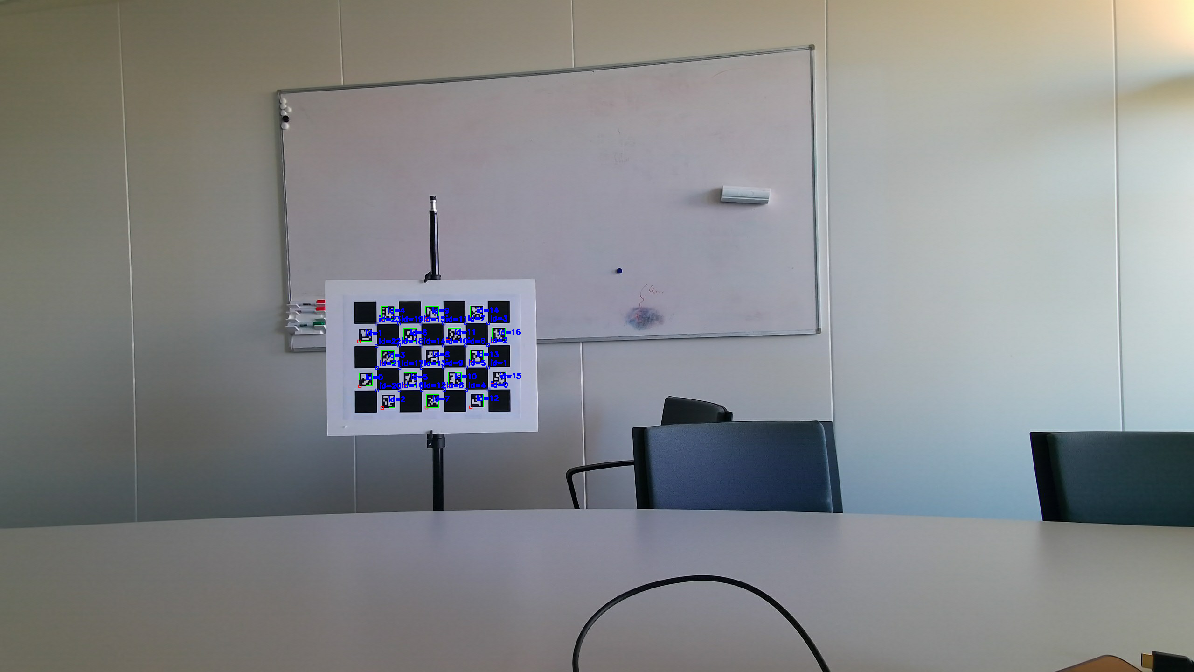
\includegraphics[width=\textwidth]{images/registration/imgl_board_detected.png}
    \caption{Chessboard detection on the left}
    \label{figure:imgl_board_detected}
  \end{subfigure}
  \caption{Detection of the chessboard corners from different position}
  \label{figure:img_board_detected}
\end{figure}


\subsubsection{Creation of a 3D point cloud of the detected corners}
\label{section:creation_3d_pc_corners}

In this second phase, the recorded positions of the corners and the depth images are used to create two 3D point clouds.

Given depth value d at (u, v) image coordinate, the corresponding 3D point is computed as follow thanks to the equation provided by\cite{Zhou2018}:

\begin{equation}
\label{equation:2dTO3d}
    \begin{array}{l}
        {z=d / c} \\
        {x=(u-c _ { x }) \cdot z / f _ { x }} \\
        {y=(v-c _ { y }) \cdot z / f _ { y }}
    \end{array}
\end{equation}
where:
\begin{itemize}
    \item $( x , y , z )$ are the coordinate of a 3D point in the corresponding camera space in a metric scale
    \item $( u , v )$ are the image coordinates
    \item $( c _ { x }, c _ { y })$ is a principal point that is usually at the image center expressed in pixel units.
    \item $ f _ { x }, f _ { y }$ are the focal lengths expressed in pixel units.
    \item $c$ is the depth scale
\end{itemize}
\leavevmode\newline
$c _ { x }, c _ { y }, f _ { x }, f _ { y }$ are the intrinsic parameters of a camera. They are different for each camera and depends of the physic of the lens. They change regarding the chosen resolution. Microsoft provides these intrinsic parameters.

The formula (\ref{equation:2dTO3d}) is applied to all the 24 detected corners in order to create a point cloud. It is done for each camera separately. Figure \ref{figure:pc_arucoboard} shows the two resulting point clouds in the same coordinate space. They are used in the next step.

\begin{figure}[H]
    \centering
    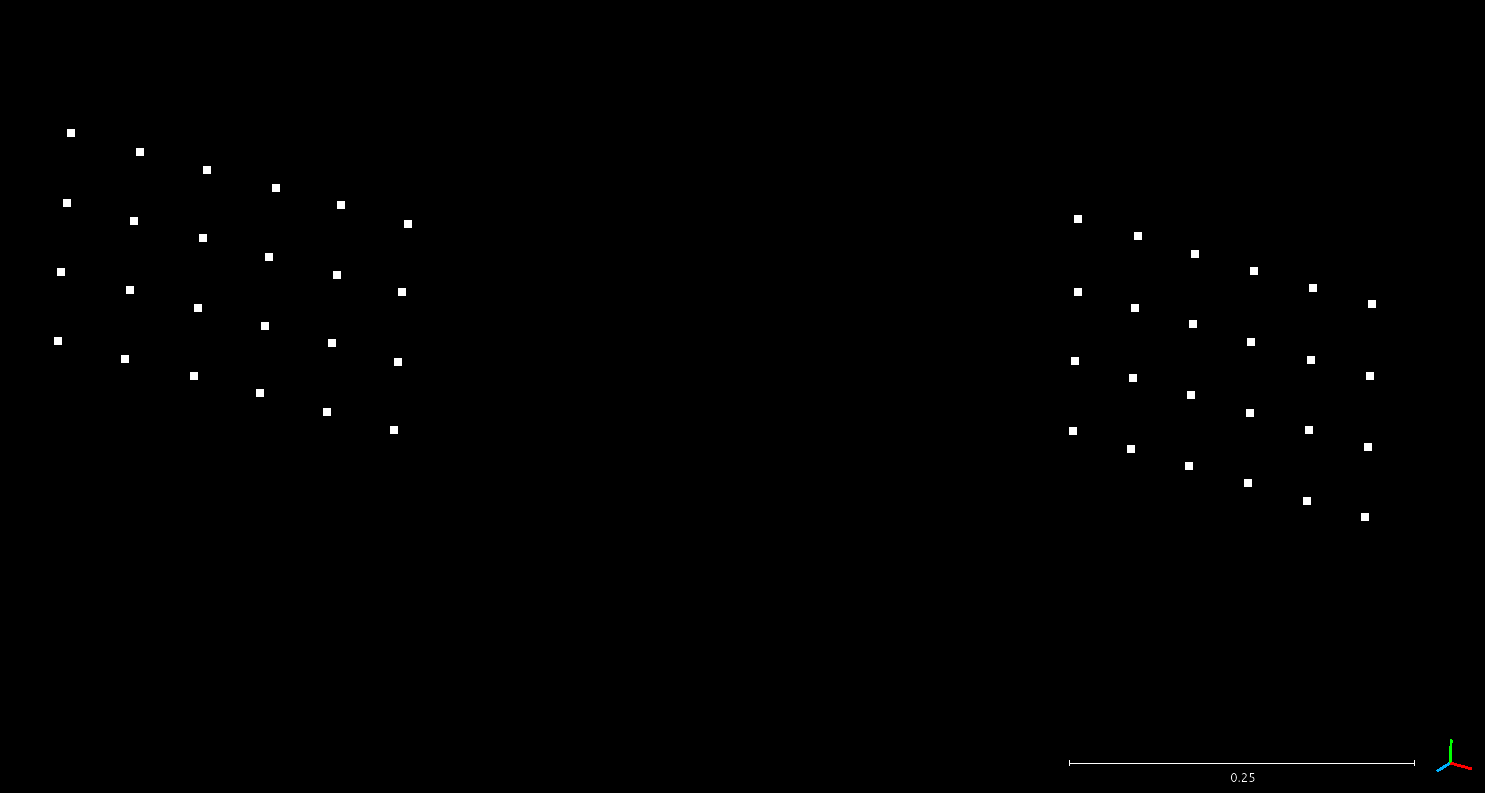
\includegraphics[width=0.65\textwidth]{images/registration/pc_aruco_24.png}
    \caption{Point cloud of the ChArUco board corners seen from the two cameras}
    \label{figure:pc_arucoboard}
\end{figure}


\subsubsection{Calculation of a 3D  rigid transformation}
\label{section:3d_rigid_transformation}

The last step consists of finding the rigid transformation to align the ChArUco board corners point clouds of the two different views. Once this matrix is found, it can be applied to the whole scene as long as the position of the cameras is not changing. The whole pipeline has to be repeated if the position of the cameras is changed. This matrix is calculated via a function\footnote{$compute\_transformation$ of the class $open3d.registration.TransformationEstimationPointToPoint$}
 provided by the library Open3D \cite{Zhou2018}. This function uses an algorithm based on \cite{umeyama_least-squares_1991}. It estimates parameters $c, \mathbf{R}$ and $\mathbf{t}$ such that the following equation is minimised:
 
%  \begin{align*}
%      \frac{1}{n} \sum_{i=1}^n\vert\vert y_i - (c\mathbf{R}x_i + \mathbf{t})\vert\vert_2^2
%  \end{align*}
 
 \begin{equation}
    \frac{1}{n} \sum_{i=1}^{n}\left\|y_{i}-\left(c \mathbf{R} x_{i}+\mathbf{t}\right)\right\|_{2}^{2}
\end{equation}

Singular value decomposition (SVD) is used by \cite{umeyama_least-squares_1991} to minimise this equation
 

% \todo{https://eigen.tuxfamily.org/dox/group__Geometry__Module.html#gab3f5a82a24490b936f8694cf8fef8e60}


% $compute\_transformation$ of the class $open3d.registration.TransformationEstimationPointToPoint$ provided by the library Open3D \cite{noauthor_open3d_nodate} is used to calculate this transformation matrix.